\documentclass[tikz]{standalone}
\usepackage{tikz}
\begin{document}
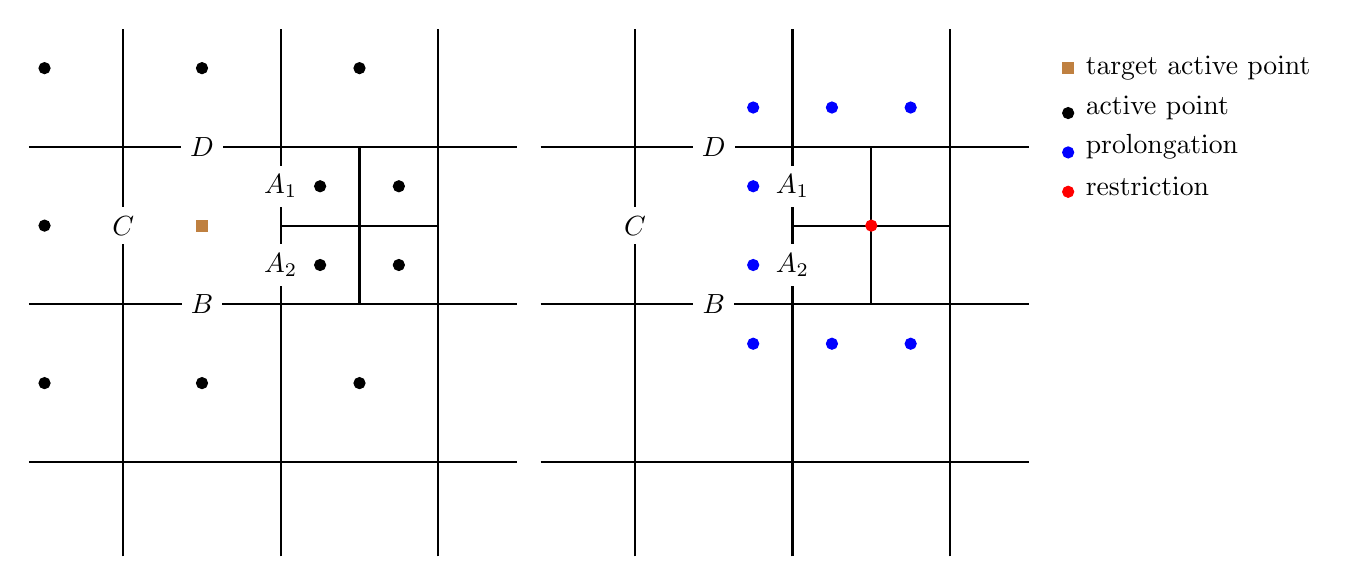
\begin{tikzpicture}
  \draw[thick,step=2cm] (-1.2,-1.2) grid (5.0,5.5); 
  \draw[thick,step=1cm] (2.0,2.0) grid (4.0,4.0); 
  \node[fill=white] at (2.0,3.5){$A_1$} ;
  \node[fill=white] at (2.0,2.5){$A_2$} ;
  \node[fill=white] at (1.0,2.0){$B$} ;
  \node[fill=white] at (0.0,3.0){$C$} ;
  \node[fill=white] at (1.0,4.0){$D$} ;
  \filldraw[brown] (1.0cm-2pt,3.0cm-2pt) rectangle (1.0cm+2pt,3.0cm+2pt);
  \filldraw[black] (1.0,1.0) circle (2pt);
  \filldraw[black] (3.0,1.0) circle (2pt);
  \filldraw[black] (-1.0,1.0) circle (2pt);
  \filldraw[black] (-1.0,3.0) circle (2pt);
  \filldraw[black] (-1.0,5.0) circle (2pt);
  \filldraw[black] (1.0,5.0) circle (2pt);
  \filldraw[black] (3.0,5.0) circle (2pt);
  \foreach \x in {2.5cm,3.5cm}
    \foreach \y in {2.5cm,3.5cm}
      \filldraw[black] (\x,\y) circle (2pt);

  \begin{scope}[xshift=6.5cm]
    \draw[thick,step=2cm] (-1.2,-1.2) grid (5.0,5.5); 
    \draw[thick,step=1cm] (2.0,2.0) grid (4.0,4.0); 
    \node[fill=white] at (2.0,3.5){$A_1$} ;
    \node[fill=white] at (2.0,2.5){$A_2$} ;
    \node[fill=white] at (1.0,2.0){$B$} ;
    \node[fill=white] at (0.0,3.0){$C$} ;
    \node[fill=white] at (1.0,4.0){$D$} ;
    \foreach \x in {1.5,2.5,3.5}
      \foreach \y in {1.5,4.5}
        \filldraw[blue] (\x,\y) circle (2pt);
    \foreach \x in {1.5}
      \foreach \y in {2.5,3.5}
        \filldraw[blue] (\x,\y) circle (2pt);
    \filldraw[red] (3,3) circle (2pt);
  \end{scope}
  \begin{scope}[xshift=12cm]
    \filldraw[brown](0.0cm-2pt,5.0cm-2pt) rectangle (0.0cm+2pt,5.0cm+2pt);
    \node[anchor=west] at (0.1, 5) {target active point};
    \filldraw[black](0.0cm,4.5cm-2pt) circle (2pt);
    \node[anchor=west] at (0.1, 4.5) {active point};
    \filldraw[blue](0.0cm,4.0cm-2pt) circle (2pt);
    \node[anchor=west] at (0.1, 4.0) {prolongation};
    \filldraw[red](0.0cm,3.5cm-2pt) circle (2pt);
    \node[anchor=west] at (0.1, 3.5) {restriction};
  \end{scope}
\end{tikzpicture}
\end{document}
